  % UTF-8 encoding
\documentclass[9pt, dvipsnames]{beamer} %
% Beamer 设置
\usetheme[secheader]{Boadilla} % 使用的 Beamer 主题: Boadilla
\usecolortheme{beaver} % 使用的 Beamer 颜色:beaver
% 字体设置
\usefonttheme{professionalfonts} % professional 字体
% 其他 Package
\usepackage{times}
\usepackage{amsmath}
\usepackage{verbatim}
\usepackage{anyfontsize}
\usepackage{subcaption} % 子图片
\usepackage{graphicx} % 图片
\usepackage[export]{adjustbox}
\setbeamertemplate{caption}[numbered]
\newcounter{saveenumi}
\resetcounteronoverlays{saveenumi}
\usepackage[multidot]{grffile} % 允许文件名带多个点
\usepackage{tabularx} % 表格
\usepackage{tikz}
\usepackage{ctex}
\usepackage{multicol}
\AtBeginSection[]
{
	\begin{frame}{Index}
		\transfade%淡入淡出效果
		\tableofcontents[sectionstyle=show/shaded,subsectionstyle=show/shaded/hide]
		\addtocounter{framenumber}{-1}  %目录页不计算页码
	\end{frame}
}
%%%%%%%%%%%%%%%%%%%

%\usepackage{ctex} % xelatex 中文

\title{Nonlinear electrodynamics coupled with gravity } % 标题
\author[林照翔]{林照翔} % 作者
\date{} % 如果 Date 参数为空,自动显示当前日期

\begin{document}
\setbeamerfont{headline}{size=\Tiny}
\everymath{\displaystyle}

    % 标题页
\begin{frame}
    \titlepage % 根据上面信息生成标题
\end{frame}

\begin{frame}
    \frametitle{\textbf{Index}}
    \begin{multicols}{2}
    \tableofcontents
    \end{multicols}
\end{frame}



\section{Aspects of a novel nonlinear electrodynamics in flat spacetime and in a gravity-coupled scenario}



\subsection{非线性电动力学模型和场方程}



\begin{frame}{麦克斯韦拉氏量和BI模型拉氏量}

麦克斯韦的拉氏量

$$
F
=\frac{1 }{2 } (B^2-E^2)
$$

$$
L_{\mathrm{maxwell}}
=-F
$$

BI 模型的拉氏量

$$
L_{\mathrm{BI}}
=\frac{2 }{\beta } \left(1-\sqrt{1+\beta F} \right) 
$$

$\beta $ 是任意常数。

弱场极限 $\beta F\ll 1 $ 下,BI 模型的拉氏量可近似为:

$$
L_{\mathrm{BI}}
=\frac{2 }{\beta } \left(1-\sqrt{1+\beta F} \right)
\approx -F + \frac{1 }{4 } \beta F^2 - \frac{1 }{8 } \beta^2 F^3 +\mathcal{O}\left(\beta^3 F^4 \right) 
$$

当 $\beta\to 0 $,BI 模型的拉氏量与线性麦克斯韦的拉氏量相同。

\end{frame}

\begin{frame}{新 NLE 模型拉氏量}
作者提出新 NLE 模型的拉氏量

$$
L_{\mathrm{general}}(F)
=-\frac{\left(aF+1 \right)^m }{\delta(bF+1)^n } \left(\beta F \right)^p
$$

$m,n,p $ 是无量纲常数,$a,b,\beta,\delta $ 是长度平方量纲的任意常数。

在弱场极限下,拉氏量可近似为:

$$
L_{\mathrm{general}}(F)
=-\frac{\left(aF+1 \right)^m }{\delta(bF+1)^n } \left(\beta F \right)^p
\approx -c\left[F^p + c_1 F^{p+1} +c_2 F^{p+2}  + \mathcal{O}\left(c_3 F^{p+3} \right) \right]
$$

$p=1 $ 时得到麦克斯韦的拉氏量。

通过分析取 $m=1,n=m+1,a=-3b $

得到含有两个参数且遵守麦克斯韦极限的拉氏量:

$$
L(F)
=\frac{\gamma(3\eta F - 1 )F }{(1+\eta F)^2 }
$$

其中,$\gamma=\beta/\delta $ 和 $\eta $ 是任意参数。

当 $\eta F\ll 1 $,即弱场极限下,拉氏量近似为:

$$
L(F)
=\frac{\gamma(3\eta F - 1 )F }{(1+\eta F)^2 } 
\approx -\gamma F + 5\gamma \eta F^2 -9\gamma \eta^2 F^3 + \gamma\mathcal{O}\left(\eta^3F^4 \right) 
$$
\end{frame}

\begin{frame}{新 NLE 模型的物理对应}
利用电位移矢量 $\vec{D} $ 与 $\vec{E} $ 的关系 $\vec{D}=\partial L/\partial \vec{E} $,可由拉氏量式得到:

$$
\vec{D}
=\gamma\frac{1-7\eta F }{(1+\eta F)^3 } \vec{E}
$$

$D_i = \varepsilon_i^{~~ j } E_j $

$$
\varepsilon_{ij} = \gamma \frac{1-7\eta F }{(1+\eta F)^3 }\delta_{ij} 
$$

磁场 $\vec{H}=-\partial L/\partial \vec{B} $ 结合拉氏量有

$$
\vec{H}
=\gamma \frac{1-7\eta F }{(1+\eta F)^3 } \vec{B}
$$

磁感应强度 $B_i=\mu_i^{~~j}H_j $

磁导率张量的逆 $\left(\mu^{-1} \right)_{ij} $

$$
\left(\mu^{-1} \right)_{ij}
=\gamma \frac{1-7\eta F }{(1+\eta F)^3 } \delta_{ij}
$$

可以认为新 NLE 拉氏量由这种特殊的介质生成。
\end{frame}

\begin{frame}{点电荷电场}
    平坦时空中拉氏量给出 E-L 运动方程:

    $$
    \partial_\mu\left(L_F F^{\mu\nu} \right) = 0
    $$
    
    其中,
    
    $$
    L_F
    \equiv \frac{\partial L }{\partial F } 
    =\frac{\gamma(-1+7\eta F) }{(1+\eta F)^3 }
    $$
    
    $F^{\mu \nu} $ 是麦克斯韦场强张量。

    可以回到无源麦克斯韦方程:

    $$
    \nabla\cdot\vec{D} = 0,\quad
    \frac{\partial \vec{D} }{\partial t } - \nabla\times\vec{H}= \vec{0} 
    $$
    
    由 Bianchi identity $\partial_\mu \tilde{F}^{\mu \nu}=0 $,$\tilde{F}^{\mu\nu} $ 是场强张量的对偶,可得
    
    $$
    \nabla\cdot\vec{B} = \vec{0},\quad 
    \frac{\partial \vec{B} }{\partial t } + \nabla\times\vec{E} = \vec{0} 
    $$    
\end{frame}

\begin{frame}
    考虑静电极限(electrostatic limit) $\vec{B}=\vec{H}=\vec{0} $,对点电荷

    $$
    \nabla\cdot\vec{D} = e\delta(\vec{r})
    $$
    
    解:
    
    $$
    \vec{D}
    =\frac{e }{4\pi r^3 } \vec{r}
    $$
    
    结合 $\vec{D},\vec{E} $ 关系和 $F=-E^2/2 $ 可得
    
    $$
    E+\frac{7 }{2 } \eta E^3
    =\frac{e }{4\gamma \pi r^2 } \left(1-\frac{\eta  }{2 } E^2 \right)^3 
    $$
    
    上式限制 $F>-1/\eta $;弱场极限 $\eta F\ll 1 $,$E(r) $ 可按 $\eta $ 展开
    
    $$
    E
    =E_{(0)} + \eta E_{(1)} + \eta^2 E_{(3)} + \mathcal{O}\left(\eta^3 \right)
    $$
    
    $E_{(1)},E_{(2)} $ 分别代表对电场 $E_{(0)} $ 的一阶和二阶修正。
\end{frame}

\begin{frame}
    比较系数可得
    
    $$
    E_{(0)}
    =\frac{e }{4\pi\gamma r^2 }
    $$
    
    $$
    E_{(1)} 
    =-\frac{7 }{2 } E_{(0)}^3 - \frac{e }{4\pi \gamma r^2 } E_{(0)}^2
    $$
    
    $$
    E_{(2)}
    =-\frac{21 }{2 } E_{(0)}^2 E_{(1)} + \frac{e }{4\pi\gamma r^2 } \left(-3E_{(0)}E_{(1)} + \frac{3 }{4 } E_{(0)}^4 \right)
    $$
    
    弱场极限下
    
    $$
    E
    \approx \frac{e }{4\pi\gamma r^2 } - 5\eta\left(\frac{e }{4\pi\gamma r^2 }  \right)^3 + \frac{273 }{4 } \eta^2\left(\frac{e }{4\pi\gamma r^2 }  \right)^5 + \mathcal{O}\left(\eta^3 \right)
    $$
    
    对于很小的 $r$ 和任意的 $\eta$,电场最大值
    
    $$
    E_{\max}
    =\sqrt{\frac{2 }{\eta } }
    $$
    
    NLE 模型中电场有限。当 $\eta\to 0 $,电场发散。
    
\end{frame}

\subsection{点电荷的能量}

\begin{frame}{点电荷的能量}
    希尔伯特应力-能量张量(Hilbert stress-energy tensor)

    $$
    T_{\mu\nu}^H
    \equiv -\frac{2 }{\sqrt{-g} } \left(\frac{\partial \left(\sqrt{-g}L(F) \right) }{\partial g^{\mu\nu} }  \right)\bigg|_{g=\eta}
    =\eta_{\mu\nu}L(F) - L_FF_\mu^\alpha F_{\nu\alpha}
    $$
    
    电能密度
    
    $$
    \rho
    =-T_t^t
    =-L_FE^2-L(F)
    =\frac{\gamma E^2\left[1+\frac{3 }{2 } \eta E^2 \left(4+\frac{\eta }{2 } E^2 \right) \right] }{2\left(1-\frac{\eta }{2 } E^2 \right)^3 } 
    $$
    
    总电能
    
    $$
    \epsilon
    =4\pi\int_{0}^{+\infty} \rho(r)r^2\mathrm{d}r
    $$ 
    
    转化为对 $E $ 的积分
    
    $$
    \epsilon
    =\frac{e^{3/2} }{\sqrt{4\pi\gamma} } \int_{0}^{\sqrt{\frac{2 }{\eta  } }} \frac{\sqrt{\left(2-\eta E^2 \right)\left[4+3\eta E^2\left(8+\eta E^2 \right) \right]\left[4+\eta E^2\left(52+21\eta E^2 \right) \right]} }{16\sqrt{E}\left(2+7\eta E^2 \right)^{5/2} } \mathrm{d}E
    $$
    
    总能量有限。当 $\eta\to 0$,点电荷自能发散。
\end{frame}

\subsection{真空双折射}

\begin{frame}{真空双折射}
        考虑平面电磁波 $(\vec{e},\vec{b}) $ 沿 $z $ 轴在两片平行电容板间传播,$x $ 轴方向有匀强电场。外电场 $\bar{\vec{E}}=(\bar{E},0,0) $,总电场 $\vec{E}=\vec{e}+\bar{\vec{E}},\vec{B}=\vec{b} $,设 $\vec{e} $ 远小于 $\bar{\vec{E}} $,拉氏量

    $$
    L\left(\vec{e}+\bar{\vec{E}},\vec{b} \right)
    =\gamma\frac{\left\{\frac{3 }{2 } \eta\left[\vec{b}^2-\left(\vec{e}+\bar{\vec{E}} \right)^2 \right] - 1 \right\}\left[\vec{b}^2-\left(\vec{e}+\bar{\vec{E}} \right)^2 \right] }{2\left\{1+\frac{\eta }{2 } \left[\vec{b}^2-\left(\vec{e} + \bar{\vec{E}}^2 \right) \right] \right\}^2 } 
    $$
    
    忽略高阶项
    
    $$
    L^{(2)}(\vec{e}+\bar{\vec{E}},\vec{b})
    =\frac{\gamma\eta\left(5+\frac{7 }{2 } \eta \bar{\vec{E}}^2 \right) }{\left(1-\frac{\eta }{2 } \bar{\vec{E}}^2 \right)^4 }\left(\vec{e}\cdot\bar{\vec{E}} \right)^2 - \frac{1 }{2 } \gamma \frac{\left(1+\frac{7 }{2 } \eta \bar{\vec{E}}^2 \right) }{\left(1-\frac{\eta }{2 } \bar{\vec{E}}^2 \right)^3 }\left(\vec{b}^2-\vec{e}^2 \right) 
    $$
    
    电位移矢量和磁场强度
    
    $$
    d_i = \frac{\partial L^{(2)} }{\partial e_i } = \left(\alpha\delta_i^j+\beta\bar{E}_i\bar{E}^j \right)e_j,\quad
    h_i
    =-\frac{\partial L^{(2)} }{\partial b_i } 
    =\alpha\delta_i^j b_j 
    $$

    $$
    \beta = \frac{2\gamma \eta\left(5+\frac{7 }{2 } \eta \bar{\vec{E}}^2 \right) }{\left(1-\frac{\eta }{2 } \bar{\vec{E}}^2 \right)^4 },\quad 
    \alpha = \gamma \frac{\left(1+\frac{7 }{2 }\eta\bar{\vec{E}}^2 \right)  }{\left(1-\frac{\eta }{2 } \bar{\vec{E}}^2 \right)^3 }
    $$
\end{frame}

\begin{frame}    
    结合关系 $d_i=\varepsilon_i^j e_j,h_i=\left(\mu^{-1} \right)_i^j b_j $
    
    $$
    \varepsilon_{ij} = \alpha\delta_{ij} + \beta\bar{E}_i\bar{E}_j ,\quad
    \left(\mu^{-1} \right)_{ij} = \alpha\delta_{ij} 
    $$
    
    平面波麦克斯韦方程
    
    $$
    k_i d^i = k_i b^i = 0,\quad
    \vec{k}\times\vec{e} = \omega\vec{b},\quad
    \vec{k}\times\vec{h} = -\omega\vec{d} 
    $$
    
    
    $$
    \left\{\varepsilon^{ijk}\varepsilon_{lmn} \left(\mu^{-1} \right)_k^l k_j k^m+\omega^2\epsilon_n^i \right\}e^n = 0
    $$
    
    $\varepsilon_{ijk} $ 是反对称张量。矩阵形式
    
    $$
    \Lambda \vec{e} = 0 
    $$
    
    $$
    \Lambda
    \equiv \begin{bmatrix}
    -k^2 \alpha+\omega^2\left(\alpha+\beta\bar{E} \right) &0 &0 \\
    0 &-k^2\alpha+\omega^2\alpha &0 \\
    0 &0 &\omega^2\alpha
    \end{bmatrix} 
    $$
    
    由 $\mathrm{det}(\Lambda)=0 $ 可知电场有两种模式。两种模式定义了色散关系。折射率定义为 $n\equiv k/\omega $,因此有两种不同的折射率
    
    $$
    n_\parallel = \sqrt{1+\frac{\beta }{\alpha } \bar{E}^2},\quad
    n_\perp = 1 
    $$
    
    不同偏振的电磁波有不同的速度 $v_\parallel=n_\parallel^{-1},v_\perp=1 $
\end{frame}

\subsection{拉格朗日量的因果性和单一性条件}

\begin{frame}{拉格朗日量的因果性和单一性条件}
    若拉氏量满足不等式:

    $$
    L_F \leqslant 0,
    L_{FF}\geqslant 0,
    L_F + 2F L_{FF} \leqslant 0
    $$
    
    则群速度不超过真空光速,且动能非负。电场部分取 $B=0 $,拉氏量 $\displaystyle{L(F)=-\frac{\left(aF+1 \right)^m }{\delta(bF+1)^n } \left(\beta F \right)^p }$ ,前两个不等式给出
    
    $$
    n\geqslant m+1,a\leqslant 0,b\geqslant 0
    $$
    
    在此基础上,第三个不等式自动满足。磁场部分取 $E=0 $,类似可得
    
    $$
    n\geqslant m+1,a\geqslant 0,b\leqslant 0
    $$
    
    $n=m+1,a=-3b $ 时的因果性和单一性条件
    
    $$
    L_F
    =\frac{\gamma\left(-1+7\eta F \right) }{\left(1+\eta F \right)^3 },
    L_{FF}
    =\frac{2\gamma \eta\left(5-7\eta F \right) }{\left(1+\eta F \right)^4 } 
    $$
    
    $$
    L_F + 2FL_{FF} 
    =\gamma \frac{-\eta F\left(26-21\eta F \right) }{\left(1+\eta F \right)^4 }
    $$
\end{frame}

\begin{frame}
    仅电场部分,取 $B=0 $,因果性和单一性条件三个不等式给出
    
    $$
    -\frac{2+7\eta E^2 }{\left(2-\eta E^2 \right)^3 } \leqslant 0,
    \frac{10+7\eta E^2 }{\left(2-\eta E^2 \right)^4 } \geqslant 0,
    \frac{-4-\eta E^2\left(521\eta E^2 \right) }{\left(2-\eta E^2 \right)^4 } \leqslant 0
    $$
    
    
    所有情况都有 $E<\sqrt{2/\eta} $,$E_{\max}=\sqrt{\eta/2} $
    
    分析磁场,取 $E=0 $,前两个不等式给出
    
    $$
    \left(-1+\frac{7 }{2 } \eta B^2 \right)\leqslant 0,
    \left(5-\frac{7 }{2 } \eta B^2 \right)\geqslant 0
    $$
    
    可以得到 $F<1/7\eta $
    
    第三不等式给出
    
    $$
    -2+\eta B^2\left(26-\frac{21 }{2 } \eta B^2 \right)\leqslant 0
    $$
    
    得到 $(13-2\sqrt{37})/21<\eta F<(13+2\sqrt{37})/21 $
\end{frame}

\subsection{新 NLE 与广义相对论的耦合}

\begin{frame}{新 NLE 与广义相对论的耦合}
    通过作用量把拉氏量 $L(F) $ 与引力进行最小耦合

    $$
    I
    =\int \mathrm{d}^4 x\sqrt{-g}\left(\frac{R }{\kappa } + L(F) \right) 
    $$
    
    其中 $R $ 为里奇标量。变分可得运动方程
    
    $$
    \nabla_\mu\left(\frac{\partial L }{\partial F } F^{\mu\nu} \right)
    =0,\quad
    R_{\mu\nu} - \frac{1 }{2 } g_{\mu\nu} R
    =\kappa T_{\mu\nu}
    $$
    
    其中 $R_{\mu\nu} $ 为里奇张量,$T_{\mu\nu} $ 为 Hilbert 能量-动量张量,在弯曲时空表达为
    
    $$
    T_\mu^\nu
    =L\delta_\mu^\nu - L_F F_{\mu\lambda} F^{\nu \lambda}
    $$
    
    考虑球对称静态时空,线元
    
    $$
    \mathrm{d}s^2
    =-f(r)\mathrm{d}t^2 + \frac{1 }{f(r) } \mathrm{d}r^2 + r^2\left(\mathrm{d}\theta^2+\sin^2\theta\mathrm{d}\phi^2 \right)
    $$
    
    假设 $F_{tr},F_{\theta\phi} $ 在 $F_{\mu\nu} $ 中非零,$F_{tr}=-F_{rt} $ 代表径向电场,$F_{\theta\phi}=-F_{\phi\theta} $ 代表径向磁场。应力能动-张量非零分量
    
    $$
    T_t^t = T_r^r
    =L(F) - L_F F_{tr}F^{tr},
    T_\theta^\theta
    =T_\phi^\phi
    =L(F) - L_F F_{\theta\phi}F^{\theta\phi}
    $$
    
    下面只关注纯磁场解和纯电场解。
\end{frame}

\begin{frame}{磁场正则黑洞解 }
    纯磁场解来自 $F_{tr=0} $,非零麦克斯韦张量分量 $F_{\theta\phi}=-q_m \sin\theta $,$q_m $ 为常数,可理解为一个磁单极子的总荷量,导致径向磁场 $B_r=q_m/r^2 $,麦克斯韦不变量 $F=q_m^2/2r^4 $;$r=0 $ 处奇异

    磁单极子能-动张量
    
    $$
    T_t^t
    =T_r^r
    =\frac{\gamma q_m^2\left(3\eta q_m^2-2r^4 \right) }{\left(2r^4+\eta q_m^2 \right)^2 }
    $$
    
    $$
    T_\theta^\theta
    =T_\phi^\phi
    =\frac{\gamma q_m^2\left(4 r^8-2\eta q_m^2 r^4+3\eta^2q_m^4 \right) }{\left(2r^4+\eta q_m^2 \right)^3 }
    $$
    
    由线元可得爱因斯坦张量
    
    $$
    G_\mu^\nu
    =\mathrm{diag}\left[\frac{f' }{r } + \frac{f-1 }{r^2 } ,\frac{f' }{r } + \frac{f-1 }{r^2 } , \frac{f'' }{2 } + \frac{f' }{r } , \frac{f'' }{2 } + \frac{f' }{r }  \right]
    $$
    
    $' $ 代表度规函数 $f(r) $ 的径向微分。爱因斯坦非线性麦克斯韦方程 $tt $ 或 $rr $ 分量简化为
    
    $$
    \frac{f' }{r } + \frac{f-1 }{r^2 } 
    =\kappa \frac{\gamma q_m^2\left(3\eta q_m^2-2r^4 \right) }{\left(2r^4+\eta q_m^2 \right)^2 }
    $$
    
    解上面方程可得度规函数
\end{frame}

\begin{frame}
    $$
    f(r)
    =1+\frac{c_0 }{r } + \frac{\kappa \gamma q_m^2 r^2 }{2r^4+\eta q_m^2 } 
    $$
    
    $c_0 $ 是积分常数。取
    
    $$
    c_0=0,
    \gamma=-\frac{2b_0^2 }{\kappa q_m^2} ,
    \eta=\frac{2g^4 }{q_m^2 }
    $$
    
    $b_0,g $ 是长度量纲常数。线元可改写为
    
    $$
    \mathrm{d}s^2
    =-\left(1-\frac{b_0^2r^2 }{r^4+g^4 }  \right)\mathrm{d}t^2 + \left(1-\frac{b_0^2r^2 }{r^4+g^4 }  \right)^{-1}\mathrm{d}r^2 + r^2\left(\mathrm{d}\theta^2+\sin^2\theta \mathrm{d}\phi^2 \right)
    $$
    
    当 $r$ 趋于无穷大,时空度规渐近平坦
    
    $$
    g_{tt}\to -1,g_{rr}\to 1 \quad \mathrm{as}\quad r\to\infty
    $$
    
    对于很小的 $r$,其行为与 de-Sitter 时空相似
    
    $$
    g_{tt}\to -\left(1-c^2r^2 \right),\quad g^{rr} \to \left(1-c^2r^2 \right)\quad \mathrm{as}\quad r\to 0
    $$
    
    $g_{tt}=0$ 给出无限红移面的位置。若度规参数满足 $0<g<0.5 b_0^2 $,则上面几何代表一系列双视界黑洞;当 $g^2=0.5b_0^2$,得到单视界黑洞;若 $g^2>0.5b_0^2$,则黑洞没有视界。特别地,当 $g^2=0$,黑洞有一个视界。
\end{frame}

\begin{frame}{曲率张量和不变量的正则性}
    可通过黎曼和里奇张量各分量是否发散来判断时空的正则性、奇异性。坐标基底,非零黎曼曲率张量分量

    $$
    R^0_{~~ 110} 
    =-\frac{b_0^2\left(3r^8 - 12 g^4 r^4 + g^8 \right) }{\left(r^4+g^4 \right)^3 } 
    $$
    
    $$
    R^0_{~~220} = R^0_{~~330} = R^2_{~~112} = R^3_{~~113}
    =\frac{b_0^2\left(r^4-g^4 \right) }{\left(r^4+g^4 \right)^2 }
    $$
    
    $$
    R^3_{~~223}
    =-\frac{b_0^2 }{r^4+g^4 } 
    $$
    
    非零 Ricci 张量分量
    
    $$
    R_{00} = -R_{11} = -\frac{b_0^2\left(r^8-12g^4r^4+3g^8 \right) }{\left(r^4+g^4 \right)^3 } 
    $$
    
    $$
    R_{22} = R_{33} = \frac{b_0^2 \left(3g^4-r^4 \right) }{\left(r^4+g^4 \right)^2 }
    $$
    
    当 $r\to 0 $,两个张量的分量都有限;当 $r\to \infty $,所有分量趋于零。
\end{frame}

\begin{frame}
    三个标量不变量:
    
    Ricci 标量
    
    $$
    R = g^{\mu\nu}R_{\mu\nu}
    =\frac{4b_0^2\left(3g^8-5g^4r^4 \right) }{\left(r^4+g^4 \right)^3 }
    $$
    
    Ricci contraction
    
    $$
    R_{\mu\nu} R^{\mu\nu}
    =\frac{4b_0^2 \left(r^{16}-14g^4r^{12}+74g^8r^8-30g^{12}r^4+9g^{16} \right) }{\left(r^4+g^4 \right)^6 }
    $$
    
    Kretschmann scalar
    
    $$
    K
    =R_{\mu\nu\lambda\delta} R^{\mu\nu\lambda\delta}
    =\frac{8\left(3g^{16}-10g^{12}r^4+74 g^8 r^8-34g^4r^{12}+7r^{16} \right)b_0^4 }{\left(r^4+g^4 \right)^6 }
    $$
    
    在 $r\to 0$ 时,三个不变量也都有限。 
\end{frame}

\begin{frame}{能量条件}
    定义 $\rho=-T_t^t,\tau=t_r^r,p=T_\theta^\theta=T_\phi^\phi $

    $$
    \rho=-\tau
    =\frac{b_0^2\left(3g^4-r^4 \right) }{\kappa \left(r^4+g^4 \right)^2 } 
    $$
    
    $$
    p
    =-\frac{b_0^2\left(3g^8-12g^4r^4+r^8 \right) }{\kappa \left(r^4+g^4 \right)^3 }
    $$
    
    NEC (Null Energy Condition) $\rho+\tau \geqslant 0,\rho+p\geqslant 0 $,第一个在 $\rho+\tau=0 $ 时自动满足;
    
    $$
    \rho+p
    =\frac{2b_0^2 r^4\left(r^4-7g^4 \right) }{\kappa \left(r^4+g^4 \right)^3 }
    $$
    
    第二个满足,只能 $r^4\leqslant 7g^4 $
\end{frame}

\begin{frame}{裸电奇点解}
    Ricci  标量

    $$
    R
    =g_{\mu\nu} R^{\mu\nu}
    =\frac{4 }{r^2 } - \frac{4f(r) }{r^2 } - \frac{8f'(r) }{r } - 2f''(r) 
    $$

    通过变量替换 $\tilde{E}=E^2$ 可以写为
    
    $$
    R
    =-8\kappa \left(L-FL_F \right)
    =-\frac{8\gamma\kappa \eta\tilde{E}^2\left(10+3\eta\tilde{E} \right) }{\left(-2+\eta\tilde{E} \right)^3 }
    $$
    
    Ricci contraction
    
    $$
    R_{\mu\nu} R^{\mu\nu}
    =8\left[\frac{f'(r) }{r } + \frac{f(r)-1 }{r^2 }  \right]^2 + 8 \left[\frac{f'(r) }{r } + \frac{f''(r) }{2 }  \right]^2
    $$
    
    $$
    \begin{aligned}
        R_{\mu\nu} R^{\mu\nu}
        &=8\kappa\left[\left(L - 2FL_F \right)^2 + L^2 \right] \\
        &=\frac{16\kappa \gamma^2 \tilde{E}^2 \left\{16+\eta \tilde{E}\left[112+\eta\tilde{E}\left(296+3\eta \tilde{E}\left(20+3\eta\tilde{E} \right) \right) \right] \right\} }{\left(-2+\eta\tilde{E} \right)^6 }
    \end{aligned}
    $$ 
    在 $\tilde{E}=2/\eta $ 或 $r=0$ 处标量发散,或者说 $r=0$ 是个时空奇点。可以计算,Kretschmann 标量 $R_{\mu\nu\lambda\delta}R^{\mu\nu\lambda\delta}  $ 在 $r=0$ 处也发散。
\end{frame}

\subsection{总结}

\begin{frame}{总结}

    新型非线性电动力学模型的有效性:
\begin{itemize}
    \item 该NLE模型引入了两个具有维度的参数,能够在弱场极限下表现出类似于Born-Infeld拉格朗日量的行为。

    \item 模型成功消除了点电荷的自能发散问题,确保了电场在某一最大值下的有限性,从而避免了传统线性电动力学中的问题。
    
    \item 在外部均匀电场的影响下,模型展示了真空双折射现象,表明其在电磁现象中的新颖性。
\end{itemize}

因果性和单一性条件:

\begin{itemize}
    \item 研究表明,在所有背景电场下,模型满足因果性和单一性条件。然而,对于磁场,因果性和单一性条件仅在有限的磁场范围内成立,这表明模型在某些情况下可能存在局限性。
\end{itemize}

引力耦合的影响:

\begin{itemize}
    \item 文章探讨了将NLE拉格朗日量与爱因斯坦广义相对论(GR)最小耦合的可能性,提出了通过引入引力场来寻找不同的时空解。

    \item 结果显示,耦合后的模型可以产生常规黑洞或裸奇点,具体取决于源是非线性磁单极子还是电荷。
\end{itemize}


时空和场奇点的挑战:

\begin{itemize}
    \item 尽管NLE模型在某些情况下能够生成常规解,但仍然存在未解决的奇点问题。文章指出,源场或几何中的奇点问题需要进一步研究,以实现时空和场奇点的同时解决。
\end{itemize}
\end{frame}

\section{Nonlinear Electrodynamics in f(T) Gravity and Generalized Second Law of Thermodynamics}



\subsection{f(T)引力和NLED基础}

\begin{frame}{f(T)引力基础}

    $f(T)$ 引力中的基本元素是四分量场 $h_a(x^\mu)$,其中英文字母标记切空间,希腊字母标记时空。$h_a=h_a^\mu\partial_\mu$,分量满足

    $$
    h_\mu^a h_b^\mu = \delta_b^a,\quad h_\mu^a h_a^\nu = \delta_\mu^\nu.
    $$

    其与度规张量 $g_{\mu\nu}$ 的关系为 $ g_{\mu\nu}=\eta_{ab}h_\mu^ah_\nu^b$,其中 $\eta_{ab}=\mathrm{diag}(1,-1,-1,-1)$ 是切空间中的闵氏度规。借助魏森博克联络 $\Gamma_{~~\mu\nu}^{\lambda}=h_a^\lambda \partial_\nu h_\mu^a$,扭率张量 $T^\rho_{~~\mu\nu}$ 和张量 $S_\rho^{~~\mu\nu}$ 可定义为

    $$
    T^{\lambda}_{~~\nu\mu} = \Gamma^\lambda_{~~\nu\mu} - \Gamma^\lambda_{~~\mu\nu} = h_a^\lambda\left(\partial_\nu h_\mu^a - \partial_\mu h_\nu^a \right),
    $$

    $$
    S_\rho^{~~\mu\nu} = \frac{1 }{2 } \left(K^{\mu\nu}_{~~~~\rho} + \delta_\rho^\mu T^{\theta\nu}_{~~~~\theta} - \delta_\rho^\nu T^{\theta\mu}_{~~~~\theta} \right),
    $$

    其中,$K^{\mu\nu}_{~~~~\rho}=-\frac{1}{2}(T^{\mu\nu}_{~~~~\rho}-T^{\nu\mu}_{~~~~\rho}-T^{\mu\nu}-T_\rho^{~~\mu\nu}) $

    $f(T)$ 引力的作用量

    $$
    S = \frac{1}{2\kappa^2}\int \mathrm{d}^4 x [ef(T)+L_m]
    $$

    其中,$e=\sqrt{-g},\kappa^2=8\pi G$,$G$ 是引力常量,$L_m$ 是宇宙中物质拉格朗日密度。
    
\end{frame}

\begin{frame}
    对作用量变分可得场方程

    $$
    \left[e^{-1}\partial_\mu \left(e S_a^{~~\mu\nu} + h_a^\lambda T^\rho_{~~\mu\lambda} S_\rho^{~~\nu\mu} \right) \right] f_T + S_a^{~~\mu\nu} \partial_\mu(T) f_{TT} + \frac{1 }{4 } h_a^\nu f
    =\frac{1 }{2 } \kappa^2 h_a^\rho T_\rho^\nu
    $$
    
    其中,$f_T=\mathrm{d}f/\mathrm{d}T,f_{TT}=\mathrm{d}^2f/\mathrm{d}T^2$,$T_\rho^\nu$ 是理想流体的能-动张量。平坦 FRW 宇宙线元

    $$
    \mathrm{d}s^2
    =\mathrm{d}t^2 - a^2(t)\left(\mathrm{d}x^2+\mathrm{d}y^2+\mathrm{d}z^2 \right),
    $$

    其中,$a$ 是依赖于时间的比例因子,相应 $h_\mu^a=\mathrm{diag}(1,a,a,a)$

    modified Friedmann equations 描述了宇宙的演化:

    $$
    12 H^2 f_T + f = 2\kappa^2 \rho_t,
    $$

    $$
    48H^2\dot{H} f_{TT} - \left(12 H^2 + 4\dot{H} \right) f_T - f= 2\kappa^2 p_t,
    $$

    其中,$H=\dot{a}/a$ 是哈勃参数,$\rho_t,p_t$ 是宇宙的总能量密度和压力。
\end{frame}

\begin{frame}{非线性电动力学基础}
    对任意物理量 $Y$,体积空间平均值定义为

    $$
    \bar{Y}
    =\lim_{V\to V_0} \frac{1 }{V } \int Y\sqrt{-g} \mathrm{d}^3 x,
    $$

    其中,$g$ 是度规行列式,$\displaystyle{V=\int\sqrt{-g}\mathrm{d}^3 x } $,电场和磁场的平均值

    $$
    \bar{E}_i = 0,\quad
    \bar{B}_i = 0,\quad
    \overline{E_i B_i} = 0,\quad
    \overline{E_i E_j} = -\frac{1 }{3 } E^2 g_{ij},\quad
    \overline{B_i B_j} = -\frac{1 }{3 } B^2 g_{ij},
    $$

    利用电磁场不变量 $F,F^*$ 来表达拉氏量,保留至二阶

    $$
    \mathcal{L}=-\frac{1 }{4 } F + \omega F^2 + \eta_0 F^{*2},
    $$

    其中,$F=F_{\mu\nu} F^{\mu\nu}=2(B^2-E^2),F^*=F_{\mu\nu}^*F^{\mu\nu}=-4\vec{E}\cdot\vec{B}$,$\omega_0,\eta_0$ 是任意常数。

    相应能-动张量

    $$
    T_{\mu\nu}
    =-4\mathcal{L}_F F_\mu^{~~\alpha} F_{\alpha\nu} + \left(F^* \mathcal{L}_{F^*} - \mathcal{L} \right) g_{\mu\nu},
    $$

\end{frame}

\begin{frame}
    结合电磁场平均值以及理想流体 $T_{\mu\nu}=(\rho+p)u_\mu u_\nu-p g_{\mu\nu}$,可得能量密度 $\rho$ 和压力 $p$

    $$
    \rho = -\mathcal{L} - 4E^2 \mathcal{L}_F,
    $$

    $$
    p = \mathcal{L} + \frac{4 }{3 } \left(E^2-2B^2 \right)\mathcal{L}_F,
    $$

    考虑等离子体中迅速衰减至零的电场,进一步有

    $$
    \rho_B = \frac{1 }{2 } B^2\left(1-8\omega B^2 \right),
    $$


    $$
    p_B = \frac{1 }{6 } B^2 \left(1-40\omega_0 B^2 \right),
    $$

    当 $\omega_0=\eta_0=0$ 时,拉氏量退化为线性麦克斯韦拉氏量,能动张量也退化

    $$
    \mathcal{L} = -\frac{1 }{4 } F,\quad
    T_{\mu\nu} = F_\mu^{~~\alpha} F_{\alpha\nu} + \frac{1 }{4 } F g_{\mu\nu}.
    $$

    对于非线性过程

    $$
    \rho = 3p = \frac{1 }{2 } \left(E^2 + B^2 \right),
    $$

    这表明宇宙由普通辐射组成,具有正压力。

\end{frame}

\subsection{宇宙学参数和热力学}

\begin{frame}{宇宙学参数}
    modified Friedmann equations 场方程可写为

    $$
    \frac{3 H^2 }{\kappa^2 } = \rho_t,\quad
    -\frac{2\dot{H} }{\kappa^2 }  = \rho_t + p_t,
    $$
    
    其中,$\rho_t=\rho_m+\rho_B+\rho_T,p_t=p_m+p_B+p_T$,下标 $m,B,T$ 分别代表物质,磁场和扭率的贡献。

    $$
    \rho_T = \frac{1 }{2\kappa^2 } \left(-12 H^2 f_T - f + 6H^2 \right),
    $$

    $$
    p_T = -\frac{1 }{2\kappa^2 } \left[48\dot{H}H^2 f_{TT} - \left(12 H^2 + 4\dot{H} \right) f_T - f + 6 H^2 + 4\dot{H} \right],
    $$

    为了方便,取 $p_m=0$,能量守恒方程

    $$
    \dot{\rho}_m + 3H \rho_m = 0,
    $$

    $$
    \dot{\rho}_B + 3H\left(\rho_B + p_B \right) = 0,
    $$

    $$
    \dot{\rho}_T + 3H\left(\rho_T + p_T \right) = 0,
    $$

\end{frame}

\begin{frame}
    第一条方程解得

    $$
    \rho_m = \rho_{m0} a^{-3},
    $$

    其中,$a_{m0}$ 是任意常量。第二条方程解得

    $$
    B=\frac{B_0}{a^2},
    $$

    其中,$B_0$ 是任意常数。这表明磁场能量密度的演化随宇宙的膨胀而衰减。

    EoS(equation of state)参数

    $$
    \begin{aligned}
        \omega_t
        &=\left\{-\frac{1 }{\kappa^2 } \left[48\dot{H}H^2 f_{TT} - \left(12 H^2 + 4\dot{H} \right) f_T - f + 6 H^2 + 4\dot{H} \right] + \frac{B^2 }{6 } \left(1-40\omega_0 B^2 \right) \right\} \\
        &\times \left\{\rho_{m0} a^{-3} + \frac{1 }{2\kappa^2 } \left[6 H^2 - f-12 H^2 f_T \right] + \frac{B^2 }{2 } \left[1-8\omega_0 B^2 \right] \right\}^{-1}
        \end{aligned}
    $$

    减速参数 $q$ 是宇宙膨胀加速度的度量,其由下式给出

    $$
    q = -1 - \frac{\dot{H} }{H^2 } .
    $$

    负的 $q$ 意味着加速状态。

\end{frame}

\begin{frame}
    当前情况下 $q_t=\frac{1}{2}(1+3\omega_t)$,于是
    $$
    \begin{aligned}
        2q_t
        &=1 + 3\left[-\frac{1 }{\kappa^2 } \left(48\dot{H} H^2 f_{TT} - \left(12 H^2 + 4\dot{H} \right) f_T - f + 6H^2 + 4\dot{H} \right) + \frac{B^2 }{6 } \left(1-40\omega_0 B^2 \right) \right] \\
        &\times \left[\rho_{m0}a^{-3} + \frac{1 }{2 } \left(6H^2-f-12H^2 f_T \right) + \frac{B^2 }{2 } \left(1-8\omega_0 B^2 \right) \right]^{-1}
    \end{aligned}
    $$

    这是 $f(T)$ 的EoS(Equation of State),可以通过几个 $f(T)$ 模型来检查这些宇宙学参数的行为。
\end{frame}

\begin{frame}{广义热力学第二定律(GSLT)}
    GLST说,在视界里和视界上的总熵不随时间减少。

    由热力学第一定律有克劳修斯关系 $-\mathrm{d}E=T_X\mathrm{d}S_X$,其中 $S_X=A/(4G)$ 是 Bekenstein 熵,$A=4\pi R_X^2$ 是视界面积,$X$ 是任意视界,$T_X=1/(2\pi R_X)$ 是霍金温度。Miao 等人发现在 $f(T)$ 引力中热力学第一定律被违背,这导致额外的熵增项 $S_P$;而在 $f_{TT}$ 很小时,热力学第一定律成立,这时熵 $S_X=(Af_T)/(4G)$,而与 $S_P$ 无关。下面采用更一般的方法来研究磁 $f(T)$ 场景下的 GSLT。熵对时间微分

    $$
    \frac{\mathrm{d}S_X }{\mathrm{d}t } + \frac{\mathrm{d}S_P }{\mathrm{d}t } = \frac{\pi R_X }{G } \left(2\dot{R}_X f_T + R_X\dot{T} f_{TT} \right).
    $$

    利用吉布斯方程找到视界熵正常熵(normal entropy) $S_I$ 的变化率

    $$
    \frac{\mathrm{d}S_I }{\mathrm{d}t } 
    =\frac{1 }{T_X } \left(\frac{\mathrm{d}E_I }{\mathrm{d}t } + p_t\frac{\mathrm{d}V }{\mathrm{d}t }  \right),
    $$

    其中,$E_I=\rho_t V,V=4\pi R_X^3/3$ 是视界体积。计算得

    $$
    \frac{\mathrm{d}S_I }{\mathrm{d}t } 
    =\frac{4\pi R_X^2 }{T_X } \left(\dot{R}_X - H R_X \right)\left(\rho_t+p_t \right).
    $$
    
\end{frame}

\begin{frame}
    总熵对时间的微分

    $$
    \begin{aligned}
        &\frac{\mathrm{d}S_X }{\mathrm{d}t } + \frac{\mathrm{d}S_P }{\mathrm{d}t } + \frac{\mathrm{d}S_I }{\mathrm{d}t } \\
        =&\frac{\pi R_X }{G } \bigg\{2\dot{R}_X f_T + R_X\dot{T}f_{TT} \\
        &+ 8\pi G R_X^2 \left[\rho_{m0}a^{-3} + \frac{1 }{\kappa^2 } \left(4\dot{H} T f_{TT} + 2\dot{H}\left(f_T-1 \right) \right) + \frac{2B_0^2 }{3a^4 } \left(1-\frac{16\omega_0 B_0^2 }{a^4 }  \right) \right] \\
        &\times \left[\dot{R}_X - H R_X \right] \bigg\}
    \end{aligned}
    $$

    GSLT认为 $(\dot{S}_X+\dot{S}_I+\dot{S}_P)\geqslant 0$,下面讨论两种常用的宇宙学视界:哈勃视界(Hubble Horizon)和事件视界(Event Horizon)。

\end{frame}

\begin{frame}{哈勃视界(Hubble Horizon)}
    假设FRW宇宙热力学系统的边界被处于平衡状态的表观视界(apparent horizon)占据。对于平坦的 FRW,它退化为半径为 $R_H$ 的哈勃视界

    $$
    R_H = \frac{1 }{H } ,\quad
    \dot{R}_H = -\frac{\dot{H} }{H^2 }
    $$

    把任意视界 $X$ 替换为 $H$ 得

    $$
    \begin{aligned}
        &\frac{\mathrm{d}S_X }{\mathrm{d}t } + \frac{\mathrm{d}S_P }{\mathrm{d}t } + \frac{\mathrm{d}S_I }{\mathrm{d}t } \\
        =&-\frac{\pi }{G H} \bigg\{\frac{2\dot{H} }{H^2 } f_T + 12\dot{H}f_{TT} +\frac{8\pi G }{H^2 }\left(1+\frac{\dot{H} }{H^2 }  \right) \\
        &\times \left[\rho_{m0}a^{-3} + \frac{1 }{\kappa^2 } \left(4\dot{H}T f_{TT} + 2\dot{H}\left(f_T-1 \right) \right) + \frac{2 B_0^2 }{3a^4 } \left(1-\frac{16\omega_0 B_0^2 }{a^4 }  \right) \right] \bigg\}.
        \end{aligned}
    $$

    这是哈勃视界上宇宙中所有流体(dust matter, magnetic and torsion contribution)总熵的变化率。
    
\end{frame}

\begin{frame}{事件视界(Event Horizon)}
    事件视界半径

    $$
    R_E = a\int_0^{\infty} \frac{\mathrm{d}t }{a } ,\quad
    \dot{R}_E = H R_E - 1.
    $$

    把任意视界 $X$ 替换为 $E$ 得

    $$
    \begin{aligned}
        &\frac{\mathrm{d}S_E}{\mathrm{d}t} + \frac{\mathrm{d}S_I}{\mathrm{d}t} + \frac{\mathrm{d}S_P}{\mathrm{d}t} \\
        =&\frac{\pi}{G} \left(a\int_t^\infty \frac{\mathrm{d}t}{a}\right)\bigg[2\left(\dot{a}\int_t^\infty -1 \right) - 12H\dot{H} \left(a\int_t^\infty \frac{\mathrm{d}t}{a}\right) \\
        &+8\pi G\times \left(a\int_t^\infty\frac{\mathrm{d}t}{a}\right)^2\left(\left(\dot{a}\int_t^\infty\frac{\mathrm{d}t}{a}-1\right)-H\left(a\int_t^\infty\frac{\mathrm{d}t}{a}\right)\right) \\
        &\times \left\{\rho_{m0}a^{-3} + \frac{1}{\kappa^2} \left(4\dot{H}T f_{TT} + 2\dot{H}(f_T-1)\right) + \frac{2B_0^2}{3a^4}\left(1-\frac{16\omega_0B_0^2}{a^4}\right) \right\} \bigg]. 
    \end{aligned}
    $$

    这代表了平衡态事件视界上宇宙中总熵的变化率。

\end{frame}

\subsection{f(T)模型的一个例子}

\begin{frame}{f(T)模型的一个例子}
    考虑如下形式的比例因子

    $$
    a(t)
    =a_0\left(t_s-t \right)^{-h},\quad
    h>0,\quad t_s\geqslant t
    $$

    哈勃参数 $H$,扭率(torsion)标量 $T$,$\dot{{H}}$ 分别为

    $$
    H = \frac{h }{t_s - t } ,\quad
    T = -\frac{6h^2 }{\left(t_s-t \right)^2 } ,\quad
    \dot{H} = \frac{h }{\left(t_s - t \right)^2 }.
    $$

    把上式代入修改 Friedmann 方程的第一条可得

    $$
    \begin{aligned}
        f(T)
        =&c_1\left(-\frac{T }{6h^2 }  \right)^{1/2} + \frac{2\kappa^2 \rho_{m0} }{a_0^3\left(3h+1 \right) } \left(-\frac{6h^2 }{T }  \right)^{3h/2} + \frac{\kappa^2 B_0^2 }{a_0^4\left(4h+1 \right) } \left(-\frac{6h^2 }{T }  \right)^{2h} \\
        &- \frac{8\kappa^2 B_0^4 \omega_0 }{a_0^8 \left(8h+1 \right) } \left(-\frac{6h^2 }{T }  \right)^{4h},
    \end{aligned}
    $$

    其中,$c_1$ 由边界条件确定。

\end{frame}

\begin{frame}
    取 $z=a_0/a - 1$,两个 EoS 参数

    $$
    \omega_t
    =\frac{20\kappa^2 B_0^4 \omega_0 }{9h^2a_0^8 } \left(1+z \right)^{(8h+2)/h} - \frac{\kappa^2 B_0^2 }{18h^2 a_0^4 } (1+z)^{(4h+2)/h} - \frac{2(3h+2) }{3h } ,
    $$

    $$
    q_t
    =\frac{10\kappa^2 B_0^4 \omega_0 }{3h^2 a_0^8 } (1+z)^{(8h+2)/h} - \frac{\kappa^2 B_0^2 }{12 h^2 a_0^4 } (1+z)^{(4h+2)/h} - \frac{5h+4 }{2h } ,
    $$

    \begin{figure}
        \centering
        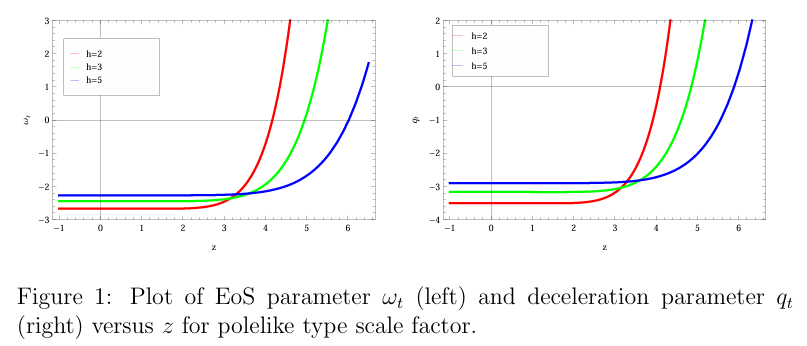
\includegraphics[width=1.0\textwidth]{img/fig1.png}
        \caption{$\omega_t$ 和 $q_t$}
    \end{figure}
    
\end{frame}

\begin{frame}

    $$
    \begin{aligned}
        f_{TT}
        &=\frac{(1+z)^{4/h} }{36h^4 } \bigg[\frac{3h(3h+2)\kappa^2\rho_{m0} }{2a_0^3(3h+1) }(1+z)^3 + \frac{2h(2h+1)\kappa^2 B_0^2 }{a_0^4(4h+1) } (1+z)^4 \\
        &- \frac{32h(4h+1)\kappa^2 B_0^4 \omega_0 }{a_0^8 (8h+1) } (1+z)^8 - \frac{c_1 }{4(1+z)^{1/h} }   \bigg].
    \end{aligned}
    $$
    \begin{figure}
        \centering
        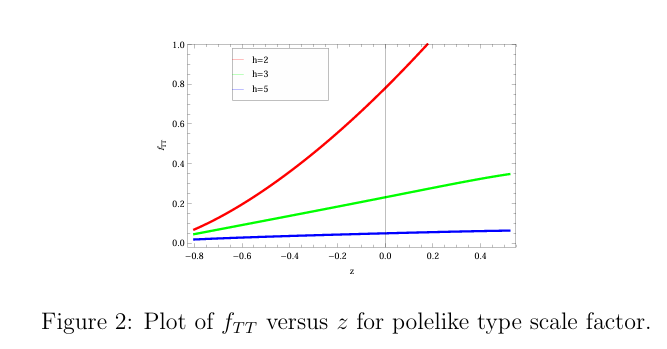
\includegraphics[width=0.8\textwidth]{img/fig2.png}
        \caption{$f_{TT}$}
    \end{figure}   
\end{frame}

\begin{frame}{Hubble Horizon}
    $$
    \begin{aligned}
        &\frac{\mathrm{d}S_H }{\mathrm{d}t } + \frac{\mathrm{d}S_I }{\mathrm{d}t } \\
        =&-\frac{\pi(1+z)^{3/h} }{Gh^3 } \bigg[\frac{3h(3h+4)\kappa^2\rho_{m0} }{2a_0^3(3h+1) }(1+z)^3 + \frac{4(h+1)\kappa^2 B_0^2 }{3a_0^4(4h+1) } (1+z)^4 \\
        &- \frac{64h(2h+1)\kappa^2 B_0^4 \omega_0 }{3a_0^8 (8h+1) } (1+z)^8- \frac{c_1 }{4h(1+z)^{1/h} } \bigg] + \frac{2\pi }{G h^3 } (1+h)(1+z)^{1/h}.
    \end{aligned}
    $$
\end{frame}

\begin{frame}{Event Horizon}
    $$
    \begin{aligned}
        &\frac{\mathrm{d}S_E }{\mathrm{d}t } + \frac{\mathrm{d}S_I }{\mathrm{d}t } \\
        =&-\frac{\pi(1+z)^{3/h} }{Gh(1+h)^2 } \bigg[\frac{(3h+4)\kappa^2\rho_{m0} }{2a_0^3(3h+1) }(1+z)^3 + \frac{4(h+1)\kappa^2 B_0^2 }{3a_0^4(4h+1) } (1+z)^4 \\
        &- \frac{64(2h+1)\kappa^2 B_0^4 \omega_0 }{3a_0^8 (8h+1) } (1+z)^8 - \frac{c_1 }{4h\kappa^2(1+z)^{1/h} } \bigg] + \frac{2\pi h }{G (1+h)^3 } (1+z)^{1/h}
    \end{aligned}
    $$

    \begin{figure}
        \centering
        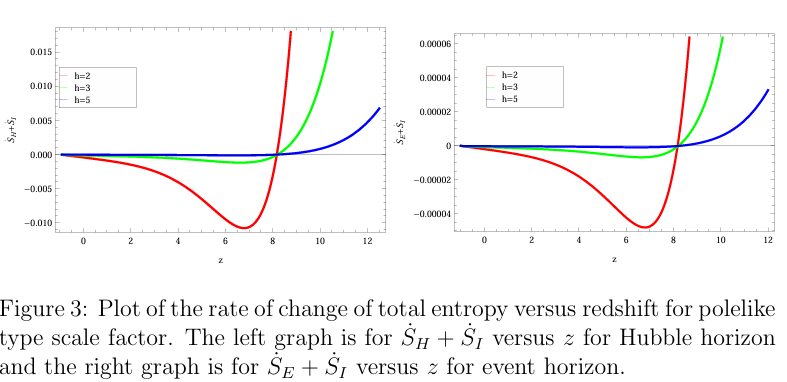
\includegraphics[width=0.7\textwidth]{img/fig3.png}
        \caption{$\dot{S}_H+\dot{S}_I$,left for Hubble Horizon,right for Event Horizon}
    \end{figure}
\end{frame}

\begin{frame}{另一种形式的比例因子}

    $a(t)=a_0(t_s-t)^h$,与之对应的 $f(T)$ 模型
    
    $$
    \begin{aligned}
        f(T)
        &=c_2\left(-\frac{T }{6h^2 }  \right)^{1/2} + \frac{2\kappa^2\rho_{m0} }{a_0^3(1-3h) } \left(-\frac{T }{6h^2 }  \right)^{3h/2} + \frac{\kappa^2 B_0^2 }{a_0^4(1-4h) } \left(-\frac{T }{6h^2 }  \right)^{2h} \\
        &- \frac{8\kappa^2 B_0^4 \omega_0 }{a_0^8(1-8h) } \left(-\frac{T }{6h^2 }  \right)^{4h},
    \end{aligned}
    $$
    \begin{figure}
        \centering
        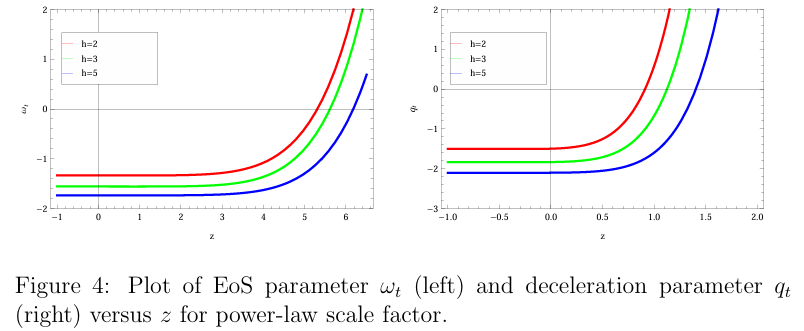
\includegraphics[width=0.7\textwidth]{img/fig4.png}
        \caption{另一种比例因子的 $\omega_t$ 和 $q_t$}
    \end{figure}
\end{frame}
    
\begin{frame}
    \begin{figure}
        \centering
        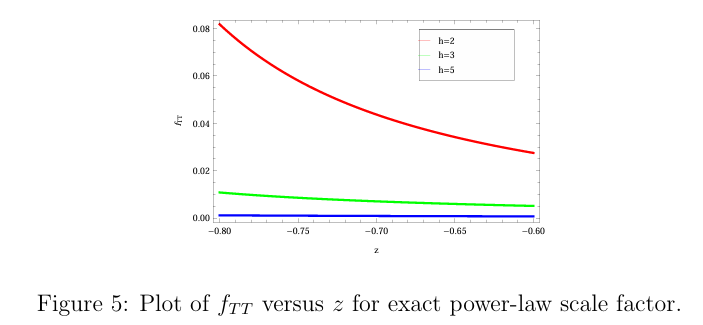
\includegraphics[width=0.6\textwidth]{img/fig5.png}
        \caption{另一种比例因子的 $f_{TT}$}
    \end{figure}
    \begin{figure}
        \centering
        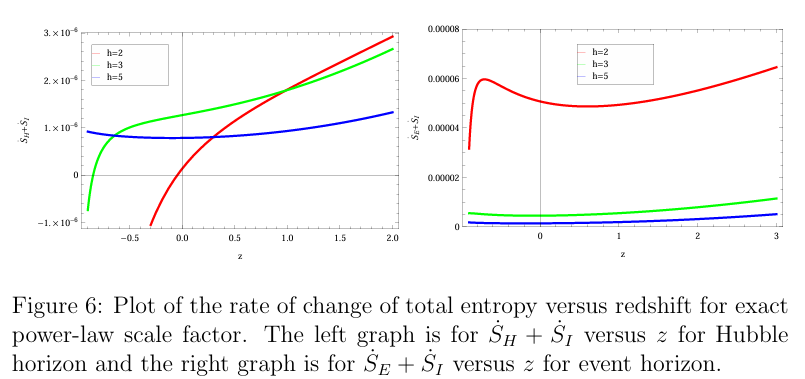
\includegraphics[width=0.6\textwidth]{img/fig6.png}
        \caption{另一种比例因子的 $\dot{S}_H+\dot{S}_I$,left for Hubble Horizon,right for Event Horizon}
    \end{figure}
\end{frame}

\subsection{总结}

\begin{frame}
    文章在包含暗能量、尘埃物质和磁场贡献的 FRW 宇宙中,在 f(T) 引力框架下研究了 NLED。采用平均手段来保留 NLED 中时空的各向同性。在这种情况下,评估了宇宙总能量密度和压力的 EoS 和减速参数。开发了哈勃和事件视界的总熵的时间导数,以使用视界熵和吉布斯方程来研究 GSLT 的合法性(validity)。使用极点和幂律形式的尺度因子构建了 f(T) 模型。讨论了一些特定模型参数的图形行为。文章的结果总结如下:


    \begin{itemize}
        \item 第一个由极点尺度因子构建的 f(T) 模型的宇宙学参数代表一个在 z≤5.6 时加速膨胀的 phamtom dominated 的宇宙。对于更高的 z 值,膨胀率降低,磁场主导扭率贡献,代表减速膨胀的宇宙。
        \item 作了哈勃和事件视界的总熵的时间导数关于 $z$ 的图,以讨论 GSLT 对满足条件 $f_{TT} \ll 1 $  的模型的合法性。对于这两个视界,GSLT 对 $z >8.2$ 和 $z <0$ 都成立。
        \item 使用精确幂律比例因子构建第二个 $f(T)$ 模型。$\omega_t$ 和 $q_t$ 关系 $z$ 的关系图表明与第一个模型相同的行为。
        \item 第二个模型也满足条件 $f_{TT}\ll 1$,以借助热力学第一定律讨论 GSLT。图6显示了哈勃视界总熵的时间导数在 $h = 2,3$ 时 $z$ 的一定范围内的正行为,而 $h = 5$ 表示 GSLT 对所有 $z$ 值的合法性。对于事件视界,GSLT 对所有 $h$ 和 $z$ 值都合法。
        \item 值得一提的是,仅对于磁宇宙,当 $z \geqslant -0.1$ 时,事件视界的总熵的时间变化率保持正值,在此范围之外变为负值。另一方面,在我们的例子中,对于具有幂律比例因子的视界,它对于磁 f(T) 框架中的所有 $z$ 值都保持在正区域。哈勃视界在两种情况下都表现出总熵的时间导数的相似行为。对于更高的红移值,宇宙学参数表明,与磁场相比,扭转贡献变得微弱。它指向宇宙的早期减速阶段。
    \end{itemize}
\end{frame}

\section{Nonlinear electrodynamics and black holes}



\subsection{NLED formalism}

\begin{frame}{电磁场不变量}
    假设非线性电磁场可由电磁势 $A_\mu$ 描述

    $$
    F_{\mu\nu}
    =2A_{[\mu,\nu]}
    $$

    $F_{\mu\nu}$ 有一个不变量和一个伪不变量

    $$
    F = \frac{1 }{4 } F_{\alpha\beta}F^{\alpha\beta},\quad
    \tilde{G} = \frac{1 }{4 } F_{\alpha\beta} \tilde{F}^{\alpha\beta} 
    $$

    其中 $\tilde{F}^{\alpha\beta}=\left(\mathrm{i}/2\sqrt{-g} \right)\varepsilon^{\alpha\beta\gamma\delta}F_{\gamma\delta}$ 是 $F^{\alpha\beta}$ 的对偶。

    若 NLED 拉氏量在洛伦兹群作用下不变,则它依赖于 $F$ 和 $\tilde{G}$;同时,在弱场极限下应与线性理论相同。
\end{frame}

\begin{frame}{$(F,\tilde{G})$ 和 $(P,\tilde{Q})$ 框架}

    两个框架可通过勒让德变换联系

    $$
    P^{\alpha\beta}
    =2\frac{\partial L }{\partial F_{\alpha\beta} } 
    =\frac{\partial L }{\partial F } F^{\alpha\beta} + \frac{\partial L }{\partial \tilde{G} } \tilde{F}^{\alpha\beta}
    $$

$$
H
=\frac{1 }{2 } P^{\alpha\beta} F_{\alpha\beta} - L\left(F,G^2 \right)
$$

与 $P^{\alpha\beta} $ 有关的不变量:

$$
P = \frac{1 }{4 } P_{\alpha\beta} P^{\alpha\beta},\quad
\tilde{Q} = \frac{1 }{4 } P_{\alpha\beta}\tilde{P}^{\alpha\beta}
$$

哈密顿方程

$$
F^{\alpha\beta}
=2\frac{\partial H }{\partial P_{\alpha\beta} } 
=\frac{\partial H }{\partial P } P^{\alpha\beta} + \frac{\partial H }{\partial Q } \tilde{P}^{\alpha\beta}
$$
    
\end{frame}

\begin{frame}
    NLED 与引力耦合作用量:

    $$
    S
    =\int \mathrm{d}^4 x\sqrt{-g} \left\{R(16\pi)^{-1}-L \right\}
    $$
    
    $R $ 是曲率标量;$g:=\mathrm{det}\left|g_{\mu\nu} \right| $
    
    $$
    L
    =\frac{1 }{2 } P^{\mu\nu}P_{\mu\nu} - H\left(P,\tilde{Q} \right)
    $$

    能动张量和曲率标量

$$
4\pi T_{\mu\nu}
=H_{,P} P_{\mu\alpha} P_\nu^\alpha - g_{\mu\nu}\left(2P H_{,P} + \tilde{Q} H_{,\tilde{Q}} - H \right)
$$

$$
R
=8\left(P H_{,P} + \tilde{Q} H_{,\tilde{Q}} - H \right) 
$$

其中,$\partial H/\partial P = H_{,P} $ 

Born-Infeld 非线性电动力学由结构函数 $H(P,\tilde{Q}) $ 给出:

$$
H = b^2\left(1-\sqrt{1-2P/b^2+\tilde{Q}^2/b^4} \right) 
$$

其中,$b $ 是最大场强,是 BI 理论中的参数。
\end{frame}

\begin{frame}{NLED能量条件}

    类时矢量 $V^\alpha,V_\alpha V^\alpha<1 $ ,local energy density 非负 $T_{\mu\nu}V^\mu V^\nu\geqslant 0 $;local energy flow 矢量是非类空的要求 $T_{\alpha\beta}T_\gamma^\alpha V^\beta V^\gamma\leqslant 0 $

    $$
    H_{,P}>0,\quad
    \left(P H_{,P} + \tilde{Q} H_{,\tilde{Q}} - H \right) \geqslant 0
    $$
    
    strong energy condition(SEC) $R_{\mu\nu}V^\nu V^\nu\geqslant 0 $,结合爱因斯坦方程得
    
    $$
    R_{\mu\nu}V^\mu V^\nu 
    =8\left(T_{\mu\nu} V^\mu V^\nu + \frac{T }{2 }  \right) \geqslant 0
    $$
    
\end{frame}

\subsection{NLED 黑洞}

\begin{frame}{NLED 黑洞}
    SSS(静态球对称) 线元

    $$
    \mathrm{d}s^2 = -\psi\mathrm{d}t^2 + \psi^{-1} \mathrm{d}r^2 + r^2\left(\mathrm{d}\theta^2+\sin^2\theta\mathrm{d}\phi^2 \right)
    $$
    
    HI发现一种解为
    
    $$
    \psi
    =1-\frac{8\pi }{r } \int_{0}^{r} \left(\sqrt{r^4+1} - r^2 \right)\mathrm{d}r
    $$
    
    上面的解有正则奇点;另一个正则解 $D_{,r}=1/r,E_{,r}=r^2/\left(r^4+1 \right) $
    
    度规函数
    
    $$
    \psi_{HI}
    =1-\frac{k }{r } + \frac{8\pi\gamma }{r } \int_{0}^{r} \left[r^2\ln\left(\frac{r^4 }{1+r^4 }  \right) \right] \mathrm{d}r
    $$

    
\end{frame}

\begin{frame}
    对 SSS 线元,PT 发现

    $$
    \psi_{PT}
    =1-\frac{d }{r } + \frac{8\pi }{r } \int_{0}^{r} H(x) x^2\mathrm{d}x
    $$

    点电荷电磁场

$$
F_{\mu\nu}
=-\frac{e }{r^2 } \frac{\partial H(P,0) }{\partial P } 2\delta_\mu^{[0}\delta_{\nu}^{r]}
$$

其中 $P=-e^2/4r^2$;若积分存在且有限,则当 $r\to 0$ 时电磁场张量是有限的;此外,当 $r$ 很大时,$H(P,0)\approx P$。这些条件保证了此解有较好的行为。

\end{frame}

\begin{frame}{BI 黑洞和 EBIon}

    SSS 时空的 EBI 解由度规函数 $\psi_{BI}(r)$ 给出
$$
\Psi_{BI}(r)
=1-\frac{2m }{r } + \frac{2 }{3 } b^2\left(r^2-\sqrt{r^4+a^4} \right) + \frac{4g^2 }{3r } G(r)
$$

$$
G'(r)
=-\left(r^4+a^4 \right)^{-1/2}
$$

其中,$m$ 是质量参数,$g$ 是磁荷,$a^4=g^2/b^2$,$b$ 是 BI 模型参数。电磁场非零分量为

$$
F_{rt}
=g\left(r^4+a^4 \right)^{-1/2},\quad
P_{rt}
=\frac{g }{r^2 }
$$

黑洞解为

$$
G(r)
=\int_{r}^{\infty} \frac{\mathrm{d}s }{\sqrt{s^4+a^4} } 
=\frac{1 }{2a } \mathbb{F} \left[\arccos\left(\frac{r^2-a^2 }{r^2+a^2 }  \right) , \frac{1 }{\sqrt{2} }  \right]
$$

其中,$\mathbb{F}$ 是第一类椭圆积分。这个解在 $r=0$ 处发散。另一方面,粒子解为

$$
G(r)
=\int_{0}^{r} \frac{-\mathrm{d}s }{\sqrt{s^4+a^4} } 
=-\frac{1 }{2a } \mathbb{F}\left[\arccos\left(\frac{a^2-r^2 }{a^2+r^2 } , \frac{1 }{\sqrt{2} }  \right) \right]
$$

这个解在 $r=0$ 处有限。

\end{frame}

\begin{frame}
    二者的联系为
$$
\int_r ^{\infty} \frac{\mathrm{d}s }{\sqrt{s^4+a^4} } + \int_0^r \frac{\mathrm{d}s }{\sqrt{s^4+a^4} } 
=\frac{1 }{a } \mathrm{K}\left[\frac{1 }{2 }  \right] 
$$

其中,$\mathrm{K}\left[\frac{1 }{2 } \right]$ 是第一类完全椭圆积分。在 $r$ 很大时,解趋于 RN 解;当 BI 模型参数 $b\to\infty$,得到线性电磁场 RN 解;在无电荷极限 $b=0$ 下,得到史瓦西黑洞解。

\end{frame}

\begin{frame}{BI黑洞中测试粒子的轨迹}

    测试粒子运动过程中有两个守恒量:能量 $E$ 和角动量 $l$;若把粒子运动限制在赤道面 $\theta=\pi/2$ 上,则可用有效势进行分析。

    对于有质量测试粒子,其轨迹由洛伦兹方程给出

    $$
    \frac{\mathrm{d}^2 x^\nu }{\mathrm{d}\tau^2 } + \Gamma_{\alpha\beta}^\nu \frac{\mathrm{d}x^\alpha }{\mathrm{d}\tau } \frac{\mathrm{d}x^\beta }{\mathrm{d}\tau } 
    =-\frac{\varepsilon }{\mu } F_{\sigma}^{\nu} \mathrm{d}x^\sigma \mathrm{d}\tau
    $$

    其中,$\varepsilon$ 是电荷量,$\mu$ 是质量,$\tau$ 是沿轨迹的仿射参数。利用两个守恒量可得

    $$
    \dot{r}^2 + \psi\left(\frac{l^2 }{r^2 } + 1 \right) - \left\{E+\frac{\varepsilon g }{\mu } \sqrt{\frac{b }{4g } } \mathbb{F} \left[\arccos\left(\frac{r^2-g/b }{r^2+g/b }  , \frac{1 }{\sqrt{2} }  \right) \right] \right\}^2=0
    $$

    与 $\dot{r}^2/2+U_{\mathrm{eff}}(E,l,r)=0$ 比较可得有效势。

    对于光子,类似有

    $$
    \dot{r}_{ph}
    =\sqrt{E^2 - \frac{\Psi_{BI} l^2 }{r^2 } \left(1+\frac{a^4 }{r^4 }  \right)^{-1}} 
    $$

    可以发现 $(\mathrm{d}r/\mathrm{d}t)_{\mathrm{photon}}<(\mathrm{d}r/\mathrm{d}t)_{\mathrm{grav}}$,即非线性效应导致光的传播速度小于引力波的传播速度。这可以解释为光子在电介质中传播导致的。
    
\end{frame}

\subsection{NLED 黑洞热力学}

\begin{frame}{NLED 黑洞热力学}
    考虑静态球对称黑洞,热力学第一定律给出

    $$
    \delta M_{\Delta} = \frac{\kappa }{8\pi } \delta a_{\Delta} + \Phi_\Delta \delta Q_\Delta
    $$

    其中,$\kappa$ 为视界处的表面引力,$M_\Delta$ 为视界质量,$a$ 为视界面积,$Q$ 为电荷,$\Phi$ 为电势;另一方面,Smarr 公式给出

    $$
    M_\Delta = \frac{\kappa a_\Delta }{4\pi } + \Phi_\Delta Q_\Delta
    $$

    Rasheed 发现,对于非线性电动力学,上面公式不适用。但可以认为

    $$
    M_\Delta = \frac{\kappa a_\Delta }{4\pi } + \Phi_\Delta Q_\Delta + V\left(a_\Delta , Q_\Delta , P_\Delta \right)
    $$

    其中,$V$ 是由视界参数决定的未知势。

\end{frame}

\begin{frame}{Bardeen 黑洞 Smarr 公式}
    Bardeen模型是爱因斯坦场方程与一种特定非线性电动力学耦合的准确解,其拉氏量为

    $$
    \mathcal{L}(F)
    =\frac{2 }{2 sg^2 } \left(\frac{2g^2 F }{1+\sqrt{2g^2 F} }  \right)^{5/2}
    $$

    其中,$g$ 是磁荷,$F$ 是电磁场不变量,$s=g/m$;对于 SSS 时空,相应度规函数为

    $$
    \psi_B
    =1-\frac{2 m(r) }{r } 
    =1-\frac{2mr^2 }{\left(r^2+g^2 \right)^{3/2} }
    $$

    Bardeen 解不含电荷,视界质量只依赖于视界面积

    $$
    M_\Delta
    =\frac{1 }{8\pi } \int\kappa \mathrm{d}a
    =\int \left(1-m' \right)\mathrm{d}r
    $$

    视界质量的正号性给出 $m(r)\leqslant r$,且 $\psi_B\geqslant 0$,这导致 $(r^2+g^2)^3\geqslant 4m^2 r^4$;$g^2=16m^2/27$ 对应极端黑洞;$g^2<16m^2/27$ 时存在内外事件视界。
\end{frame}

\begin{frame}
    Bardeen 黑洞的势 $V$ 是不确定的,除非把一个积分常数设为零,于是
    
    $$
    V = m r^3 \frac{2g^2 - r^2 }{\left(g^2 + r^2 \right)^{3/2} }
    $$

    代入 Smarr 公式得到

    $$
    M_\Delta = \frac{r }{2 } - \frac{m r^3 }{\left(r^2+g^2 \right)^{3/2} } 
    $$

    注意到,Bardeen 黑洞的视界质量只依赖于视界面积,这是因为磁荷被认为是视界的不变参数。
    \begin{figure}
        \centering
        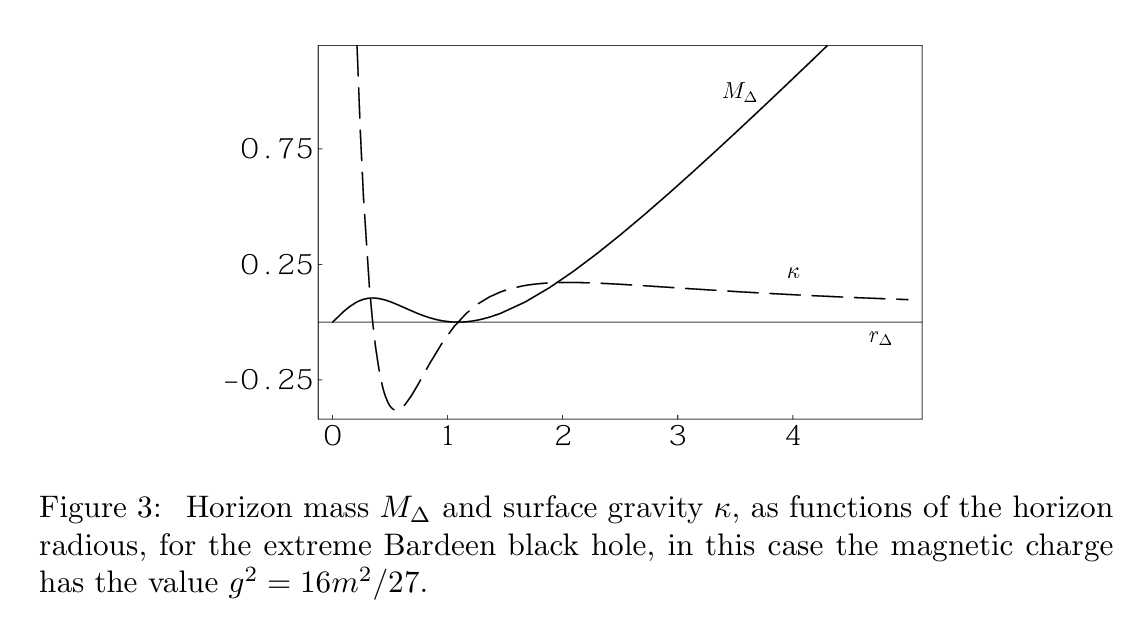
\includegraphics[width=0.5\textwidth]{img/fig7.png}
        \caption{$M_\Delta$ 和 $\kappa$}
      \end{figure}
\end{frame}

\subsection{孤立视界框架和质量关系}

\begin{frame}{孤立视界框架和质量关系}
    ADM模型中,带毛黑洞(hairy black hole)可以被视为普通黑洞和孤立子的束缚态。下面的公式将有色黑洞解的视界质量与相应理论的孤立子解的ADM质量联系起来

    $$
    M_{\mathrm{sol}}^{(n)} = M_{\mathrm{ADM}}^{(n)} - M_\Delta^{(n)} 
    $$

    若EBI理论给出两个确定解:黑洞解和孤子解,那么即使 EBI 黑洞是无色的(is not a coloured one),我们也应当采用 ACS 模型,认为 $b$ 是一个自由参数。因此这里 $n$ 应该替换为 BI 参数 $b$(分立或连续)。 

    EBI 解中,视界质量和 ADM 质量是视界半径 $r_\Delta$ 的函数,它们分别为

    $$
    M_\Delta^{(b)}(r_\Delta)
    =\frac{r_\Delta }{2 } + \frac{b^2 r_\Delta }{3 } \left(r_\Delta^2 - \sqrt{r_\Delta^4 + a^4} \right) - \frac{2g^2 }{3 } \int_0^{r_\Delta} \frac{\mathrm{d}s }{\sqrt{a^4+s^4} } 
    $$

    $$
    M_{\mathrm{ADM}}^{(b)}(r_\Delta)
    =\frac{r_\Delta }{2 } + \frac{b^2 r_\Delta }{3 } \left(r_\Delta^2 - \sqrt{r_\Delta^4 + a^4} \right) + \frac{2g^2 }{3 } \int_{r_\Delta}^{\infty} \frac{\mathrm{d}s }{\sqrt{a^4+s^4} }
    $$

    由于大多数 ACS 特征得到了满足,可以认为,当保持电荷不变而变化 BI 参数 $b$ 时,EBI 理论的静态部分可以用 Ashtekar 等人提出的有色黑洞(colored black hole)的启发式(heuristic)模型来描述。

\end{frame}

\begin{frame}
    \begin{figure}
        \centering
        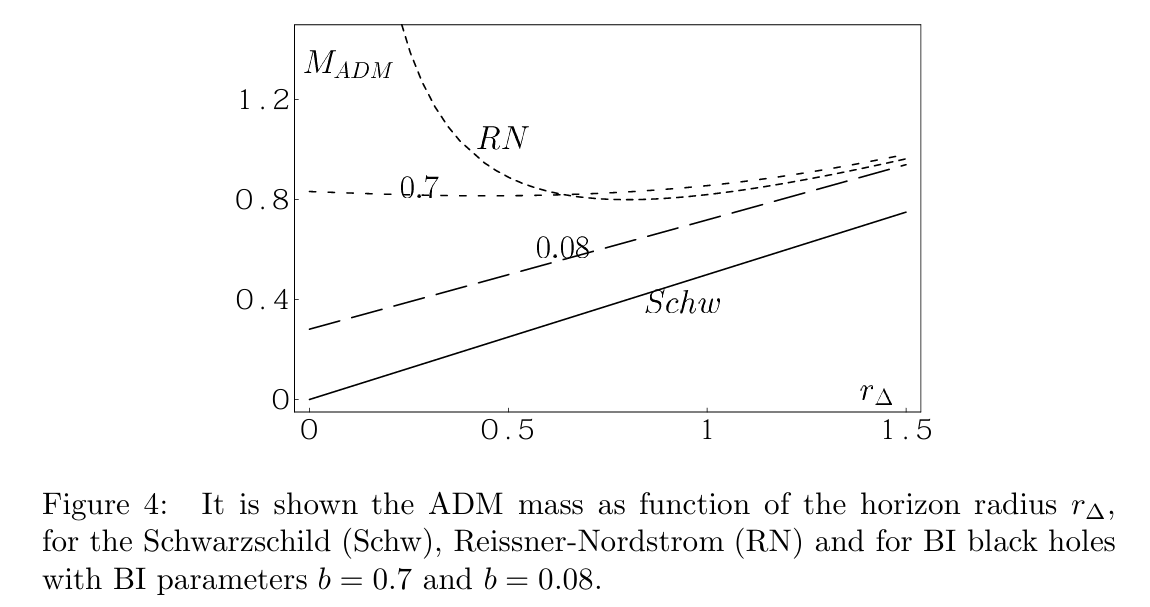
\includegraphics[width=0.8\textwidth]{img/fig8.png}
        \caption{ADM mass compared with Schw, RN, and BI black holes}
    \end{figure}
\end{frame}

\subsection{NLED 黑洞的稳定性}

\begin{frame}{稳定性条件}
    稳定性条件是一些对拉氏量及其微分 $L(F),L_F,L_{FF}$ 的约束。变量替换 $y=\sqrt{2g^2 F}$ 后可表述为
    $$
    L(y)>0,\quad
    L(y)_{,y}>0,\quad
    L(y)_{,yy}>0 
    $$

    $$
    f(y)
    \equiv yL_{,yy} / L_{,y} > 0,\quad
    f(y) N(y) < 3    
    $$

    其中,$N(y)$ 为 SSS 线元度规函数。BI 拉氏量满足稳定性条件。把 BI 拉氏量写作 $y$ 的函数,取 $\tilde{G}=0$ 得

    $$
    L(y)
    =b^2\left(\sqrt{1+\frac{y^2 }{b^2 g^2 } } - 1 \right) > 0 
    $$

    其他不等式
    
    $$
    L_{,y} = \frac{y }{g^2 } \left(1 + \frac{y^2 }{b^2 g^2 }  \right)^{-1/2} > 0
    $$

    $$
    L_{,yy} = \frac{1 }{g^2 } \left(1 + \frac{y^2 }{b^2 g^2 }  \right)^{-3/2} > 0
    $$

    $$
    f(y) = y\frac{L_{,yy} }{L_{,y} } = \left(1 + \frac{y^2 }{b^2 g^2 }  \right)^{-1} > 0
    $$

\end{frame}

\begin{frame}
    对于所有 $y$,以上不等式均成立。考虑不等式 $f(y)N(n)<3$,由于 $0<f(y)\leqslant 1$,则其化简为 $\psi_{BI}(y)<3$

    对于黑洞情况,度规函数

    $$
    \psi_{BI}(y)
    =1-\frac{2m\sqrt{y} }{g } + \frac{2b^2 g^2 }{3y } \left(1-\sqrt{1+\frac{y^2 }{b^2 g^2 } } \right) + \frac{2\sqrt{gby} }{3 } \mathbb{F}\left[\arccos\left(\frac{gb-y }{gb+y } \right), \frac{1 }{\sqrt{2} }   \right] 
    $$

    在 $0<y<y_\Delta=8.35$ 范围内,$0<\psi_{BI}(y)\leqslant 1$,不等式得以满足。

    对于 EBI 方程类粒子解,度规函数

    $$
    \psi_{BI}(y)
    =1-\frac{2m\sqrt{y} }{g } + \frac{2b^2 g^2 }{3y } \left(1-\sqrt{1+\frac{y^2 }{b^2 g^2 } } \right) - \frac{2\sqrt{gby} }{3 } \mathbb{F}\left[\arccos\left(\frac{y-gb }{gb+y } \right), \frac{1 }{\sqrt{2} } \right]
    $$

    $N(y=0)=1$,而 $N(y)$ 单调递减,因此 $N=\psi<3$ 总能满足。

    因此,EBI 的黑洞解和类粒子解都是稳定的。

\end{frame}
    
\begin{frame}[noframenumbering]
    \centering
    {\fontsize{40}{50}\selectfont Thank You!}
\end{frame}

\end{document}